\setcounter{page}{1}
\section*{Zielsetzung}
Im Versuch 355 \emph{Gekoppelte Schwingkreise} soll das Verhalten gekoppelter schwingungsfähiger Systeme untersucht werden. Hierzu
werden zwei kapazitiv gekoppelte elektrische Schwingkreise verwendet.
\section{Theorie}
Der prinzipielle Aufbau ist in Abb. \ref{fig: prinz_schwingkreis} einzusehen. Unter Anwendung der Kirchhoffschen Regeln erhält man folgendes gekoppletes
Differentialgleichungssystem für die Ströme $I_1$ und $I_2$:
\begin{align}
\begin{aligned}
L \, \ddot{I}_1 + \frac{1}{C} \, I_1 + \frac{1}{C\ua{k}} \left(I_1 - I_2 \right) &= 0 \\
L \, \ddot{I}_2 + \frac{1}{C} \, I_2 + \frac{1}{C\ua{k}} \left(I_1 - I_2 \right) &= 0 \\
\end{aligned}
\end{align}

\begin{figure}
  \centering
  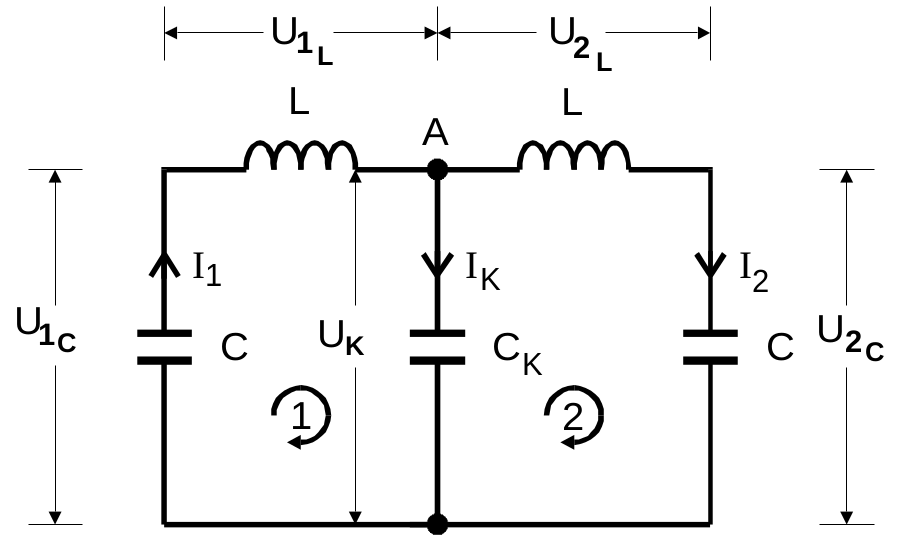
\includegraphics[width = 6cm]{pics/prinzip_schwingkreis.png}
  \caption{Prinzipschaltbild zweier kapazitiv gekoppelter Schwingkreise \cite{anleitung355}}
  \label{fig: prinz_schwingkreis}
\end{figure}

Eine Hauptachsentransformation des Systems erhält man trivialerweise durch Addition bzw.
Subtraktion der beiden Gleichungen:
\begin{align}
\begin{aligned}
  L\,\frac{\dif{}^2}{\dif{t}^2} \left( I_1 + I_2 \right) + \frac{1}{C} \left( I_1 + I_2 \right) &= 0 \\
  L\,\frac{\dif{}^2}{\dif{t}^2} \left( I_1 - I_2 \right) + \left(\frac{1}{C} + \frac{2}{C\ua{k}}\right) \left( I_1 - I_2 \right) &= 0 \\
  \label{eq: gekoppeltes_lgs}
\end{aligned}
\end{align}
Die Relativgröße $\left( I_1 + I_2 \right)$ schwingt also harmonisch mit den Frequenzen:

\begin{equation}
  \nu^+ = \frac{1}{2\pi \, \sqrt{LC}}
  \label{eq: nu+}
\end{equation}

Die Größe $\left( I_1 - I_2 \right)$ entsprechend mit der Frequenz:

\begin{equation}
\nu^- = \frac{1}{2\pi \, \sqrt{L\, \left(\frac{1}{C} + \frac{2}{C\ua{k}}\right)^{-1}}}
\label{eq: nu-}
\end{equation}

Die beiden Frequenzen entsprechen genau jenen Frequenzen der Fundamentalschwingungen: Gleich- und gegenphasige Schwingung bei
betragsmäßig gleichen Anfangsamplituden (in Analogie zum gekoppelten Pendel aus der Mechanik). Allgemein gilt $\nu^+ < \nu^-$.\\
Alle weiteren Lösungen des Systems \eqref{eq: gekoppeltes_lgs} erhält man durch Superposition. Wird lediglich der linke Schwingkreis zu Schwinungen
angeregt, so entstehen sogenannte Schwebungsvorgänge, die im Versuch untersucht werden sollen. Hierbei oszilliert die Energie des gekoppelten Systems
mit der Schwebungsfrequenz $\nu\ua{schwebe}$ zwischen den Schwingsystemen.
\begin{equation}
  \nu\ua{schwebe} = \nu^- - \nu^+
  \label{eq: nu_schwebe}
\end{equation}
Innerhalb dieser enhüllenden Schwingung der einzelnen Amplituden führen die Oszillatoren die Schwingungsfrequenz $\nu\ua{schwing}$ aus.

\begin{equation}
  \nu\ua{schwing} = \nu^- + \nu^+
  \label{eq: nu_schwing}
\end{equation}\par

Wird das System im linken Zweig des Aufbaus durch eine Wechselspannung mit Amplitude $\left| U \right|$ und Frequenz $\omega$ angeregt, so ergibt sich für den Betrag des
Stroms $I_2$:
\begin{equation}
|I_2(\omega)| = |U| \left( 4 \omega^2 C\ua{K}^2 R^2 Z(\omega )^2 + \left(\frac{1}{\omega C\ua{K}} - \omega C\ua{K} Z(\omega )^2 + \omega R^2 C\ua{K}\right)\right)^{-\frac{1}{2}}
\label{eq: I_2(omega)}
\end{equation}
Hierbei entspricht $R$ einem in beiden Zweigen des Aufbaus geschalteten ohmschen Widerstand und $Z(\omega)$ der Vereinfachung:
\begin{equation}
  Z(\omega ) \coloneqq \omega L - \frac{1}{\omega } \left(\frac{1}{C} + \frac{1}{C\ua{K}}\right)
\end{equation}
Der Strom $I_2$ erreicht Maxima für die Fundamentalfrequenzen $\omega^+$ bzw. $\omega^-$. Diese Gegebenheit wird im Versuch ausgenutzt um
die Fundamenatlschwinungen experimentell zu bestimmen.
